%! TeX root = ../../*.tex

\currentpaper[https://doi.org/10.1111/j.1365-246X.2006.03191.x]{tape2007finite}

\begin{frame}[c]{\titleprefix: Selection of the trial step}

  \centering

  \begin{minipage}{0.4\textwidth}
    \tiny
    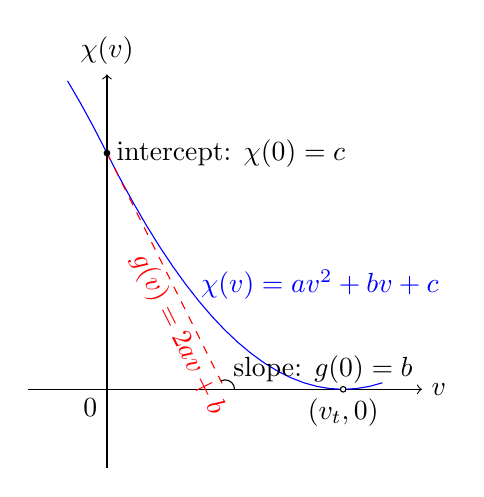
\begin{tikzpicture}[domain = -0.5:3.5]
      % axes
      \draw[->] (-1, 0) -- (4, 0) node[right] {$v$};
      \draw[->] (0, -1) -- (0, 4) node[above] {$\chi(v)$};
      \draw (0, 0) node[below left] {$0$};
      % curve
      \draw[color = blue] plot (\x, {1.0/3*\x^2 - 2*\x + 3});
      \node[blue, right = 2pt] at (1.0, 1.33) {$\chi(v) = av^2 + bv + c$};
      % tangent line
      \draw[red, dashed] (0, 3) -- (1.5, 0);
      \node[red, rotate = - atan(2.0)] at (0.9, 0.7) {$g(v) = 2av + b$};
      \draw[thin] (1.5, 0) +(0:0.12) arc (0:{180 - atan(2.0)}:0.12)
        node[above = 4pt, right = 1pt] {slope: $g(0) = b$};
      % sample points
      \draw[fill = black] (0, 3) circle(1pt)
        node[right] {intercept: $\chi(0) = c$};
      \draw[black, fill = white] (3, 0) circle(1pt)
        node[below] {$(v_t, 0)$};
    \end{tikzpicture}
  \end{minipage}
  %
  \hspace{0.5cm}
  %
  \begin{minipage}{0.4\textwidth}
    \tiny
    Interpolate $\chi(v)$ using a quadratic polynomial to compute
    an analytic minimum, a test model location $v_t$ at which the value
    and slope of $\chi(v)$ are both zero.
    At the extremal point:
    \[ 0 = \frac{4ac - b^2}{4a} \Rightarrow a = \frac{b^2}{4c} \]
    \[ v_t = - \frac{b}{2a} = - \frac{2c}{b} = - \frac{2 \chi(0)}{g(0)} \]

    \begin{figureblock}{Modified from Figure 11(d)}
      The misfit is denoted by the $\bullet$,
      and the gradient is denoted by the red dashed line.
      The white circle indicates the test model obtained by quadratic
      extrapolation of the gradient through $\chi = 0$.
    \end{figureblock}
  \end{minipage}

\end{frame}
